\section{Finite Element Analysis}

This section of the lab examines several different truss designs using finite element analysis.
Sample 2D truss designs were evaluated using a provided MATLAB program in order to determine the axial forces and deflections in each member of the truss when various loads were applied. 
These sample designs, referenced by a design number throughout this report, are shown in figure \ref{fig:designs_given}.
The strengths and weaknesses of these truss designs are discussed. 
The load/deflection characteristics and the efficiency (stiffness/weight) of each structure is examined and used to compare each design.
Five additional designs are considered and compared to those provided on the basis of overall efficiency.
Finally, the results of an analytical solution, calculated using the method indeterminate structures, is presented and compared to the numerical approximations generated by the finite element analysis.

 \begin{figure*}[p]
    \centering
    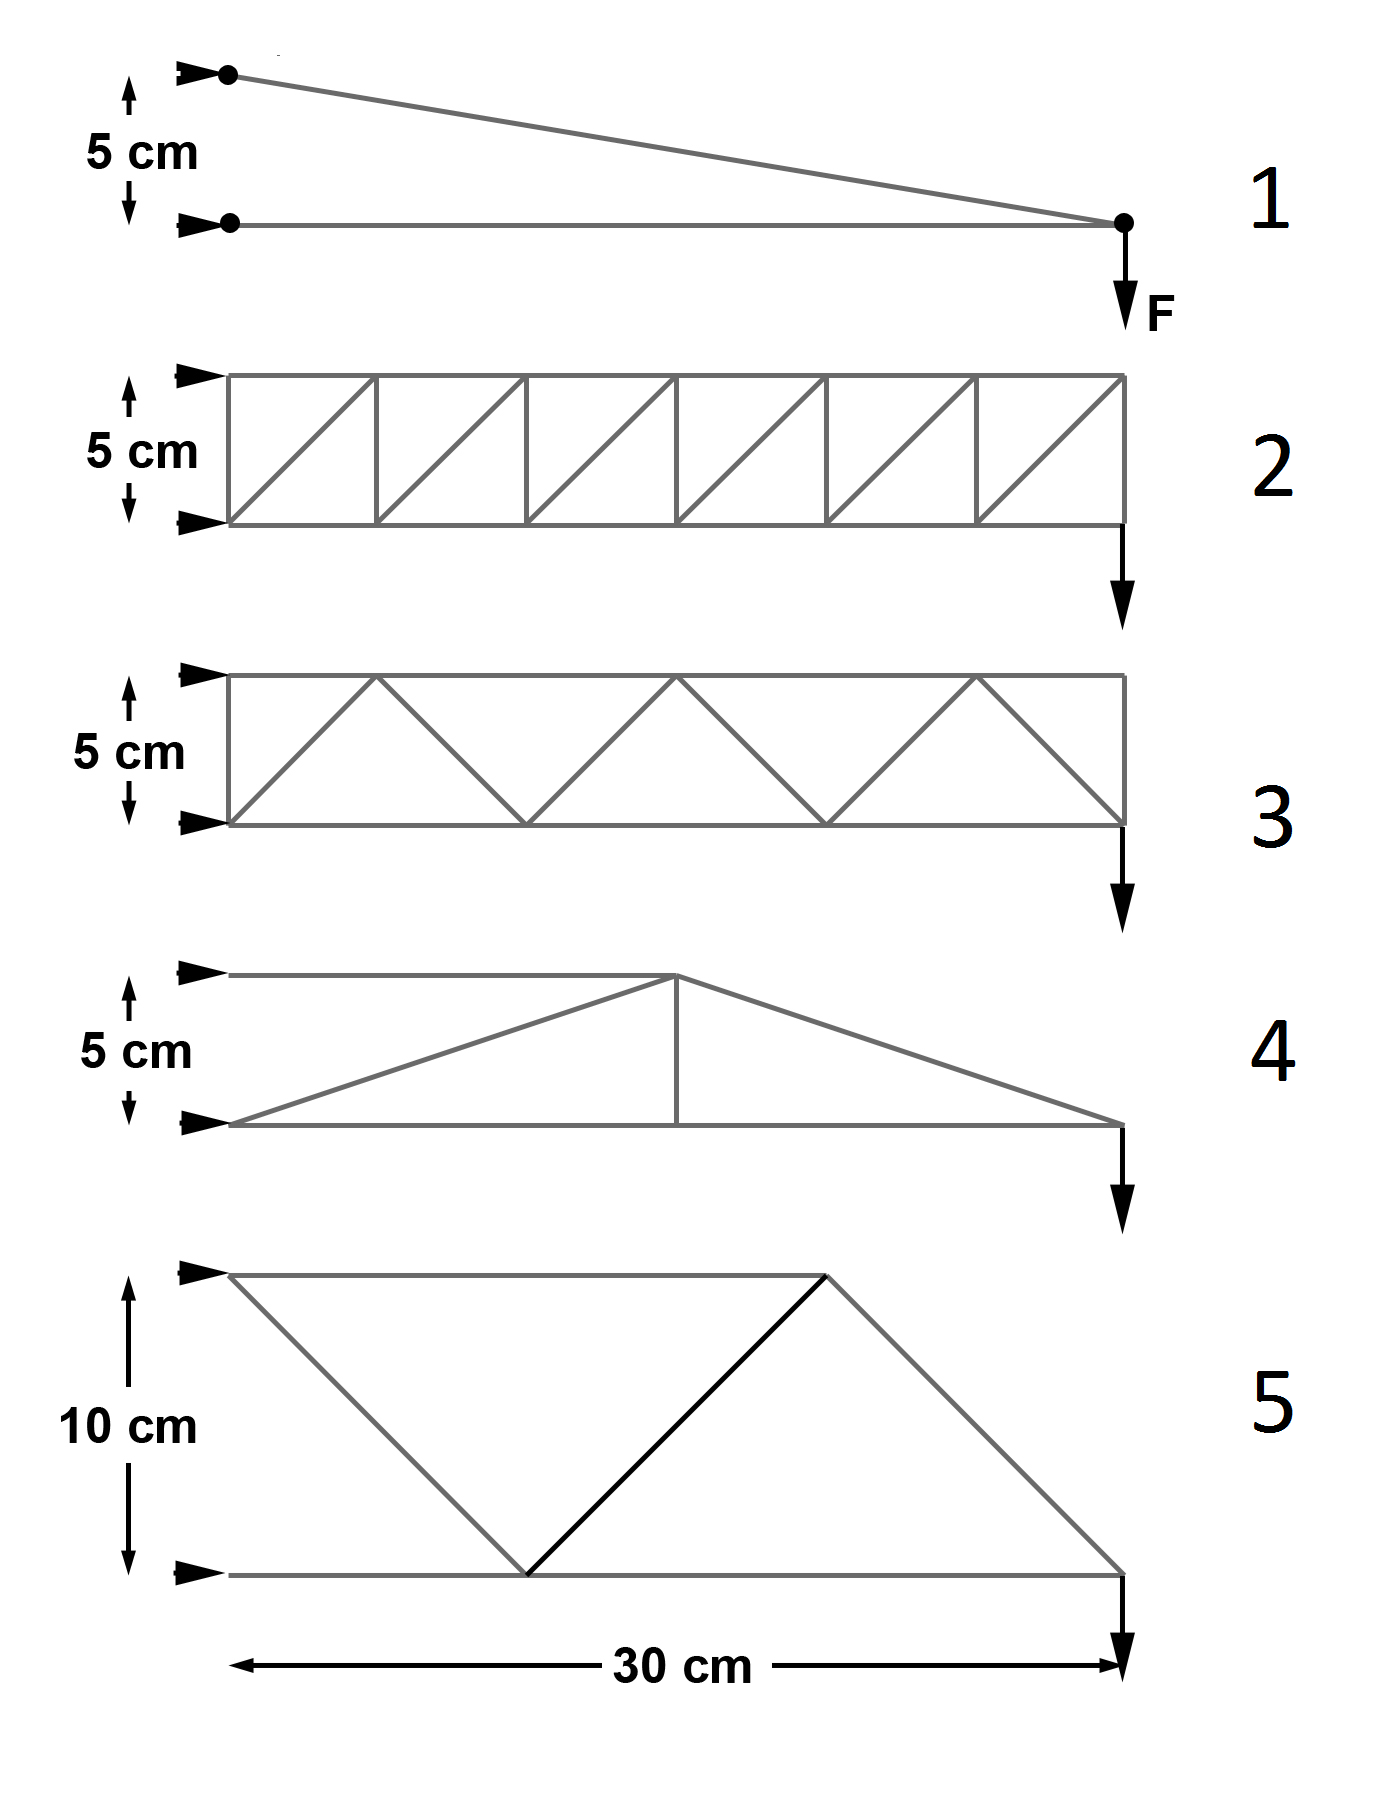
\includegraphics[width=0.45\textwidth]{images/designs_given}
    \caption{Provided Designs With Reference Numbers}
    \label{fig:designs_given}
\end{figure*}

\subsection{Methods and Results}

	\subsubsection{Basic results}
%Deflection, max tension, max compression under loads of 1/30/50 N for E of 96, 103 and 110 GPa

Table \ref{tbl:initalresults} shows initial results of the finite element analysis for each of the provided five designs.
The overall deflection in addition to the maximum tension and compression of any member is provided for a varying range of Young's modulus.
Furthermore, table \ref{tbl:forcesdesign2} lists the deflection and maximum tension and compression in any member for design two over a range of applied forces.

\begin{table*}[hp]
	\centering
	\caption{Initial Results, Deflection for 1 N, and Effect of Young's Modulus}
	\label{tbl:initalresults}
	\vspace{6pt}
	\begin{tabular}{ccc}
		%\toprule
		%Design & E & Max Tension (Stress) & Max Compression (Stress) & Deflection \\
		%\midrule
		% & 96 & 7.683e+005 &  -7.578e+005 & 0.029 mm \\
		%1 & 103 & 7.683e+005 &  -7.578e+005 & 0.027 mm \\
		% & 110 & 7.683e+005 &  -7.578e+005 & 0.025 mm \\
		%\midrule
		 %& 96 & ? & ? & 0.0112 mm \\
		%2 & 103 & ? & ? & 0.0103 mm \\
		% & 110 & ? & ? & 0.0097 mm \\
		%\midrule
		% & 96 & ? & ? & 0.0107 mm \\
		%3 & 103 & ? & ? & 0.010 mm\\
		% & 110 & ? & ? & 0.0094 mm \\
		%\midrule
		% & 96 & ? & ? & 0.0148 mm \\
		%4 & 103 & ? & ? & 0.0138 mm \\
		% & 110 & ? & ? & 0.0129 mm \\
		%\midrule
		% & 96 & ? & ? & 0.0036 mm \\
	%	5 & 103 & ? & ? & 0.0034 mm \\
	%	 & 110 & ? & ? & 0.0032 mm \\
	%	\bottomrule
		\toprule
		Design & E & Deflection \\
		\midrule
		 & 96 & 0.029 mm \\
		1 & 103 & 0.027 mm \\
		 & 110 & 0.025 mm \\
		\midrule
		 & 96 & 0.0112 mm \\
		2 & 103 & 0.0103 mm \\
		 & 110 & 0.0097 mm \\
		\midrule
		 & 96 &  0.0107 mm \\
		3 & 103 & 0.010 mm\\
		 & 110 & 0.0094 mm \\
		\midrule
		 & 96 & 0.0148 mm \\
		4 & 103 & 0.0138 mm \\
		 & 110 & 0.0129 mm \\
		\midrule
		 & 96 &  0.0036 mm \\
		5 & 103 &  0.0034 mm \\
		 & 110 & 0.0032 mm \\
		\bottomrule
	\end{tabular}
\end{table*}

\begin{table*}[hp]
	\centering
	\caption{Force Variation - Design Two (E = 100 GPa)}
	\label{tbl:forcesdesign2}
	\vspace{6pt}
	\begin{tabular}{cccc}
		\toprule
		Applied force & Maximum Tension (Force) & Maximum Compression (Force) & Endpoint Deflection \\
		\midrule
		10 N & 60 N & 50 N & 0.107 mm \\
		20 N & 120 N & 100 N & 0.214 mm \\
		30 N & 180 N & 150 N & 0.320 mm \\
		40 N & 240 N & 200 N & 0.427 mm \\
		\bottomrule
	\end{tabular}
\end{table*}


%TRUSS #2 (E= 100e9, F=10N)
%****Nodal Displacement Result******
%-9.473e-006   -1.067e-004   0.000e+000
%****Element Result******
% Elem     AXFORCE        AXSTRESS   
%    1    -5.000e+001        -6.315e+006   
%    2    -4.000e+001        -5.052e+006    
%    3    -3.000e+001        -3.789e+006    
%    4    -2.000e+001        -2.526e+006    
%    5    -1.000e+001        -1.263e+006    
%    6    2.842e-014          3.590e-009    
%    7    1.000e+001           1.263e+006    
%    8    2.000e+001           2.526e+006    
%    9    3.000e+001           3.789e+006   
%   10    4.000e+001          5.052e+006   
%   11    5.000e+001         6.315e+006    
%   12    6.000e+001         7.578e+006     
%   13    7.388e-007         9.331e-002     
%   14    -1.414e+001      -1.786e+006     
%   15    1.000e+001        1.263e+006     
%   16    -1.414e+001      -1.786e+006     
%   17    1.000e+001         1.263e+006     
%   18    -1.414e+001      -1.786e+006    
%   19    1.000e+001         1.263e+006    
%   20    -1.414e+001      -1.786e+006     
%   21    1.000e+001       1.263e+006     
%   22    -1.414e+001       -1.786e+006     
%   23    1.000e+001        1.263e+006    
%   24    -1.414e+001      -1.786e+006     
%   25    1.000e+001         1.263e+006     
%
%TRUSS #2 (E= 100e9, F=20N)
%****Nodal Displacement Result******
% 7   -1.895e-005   -2.134e-004
% Elem     AXFORCE        AXSTRESS    
%    1    -1.000e+002     -1.263e+007    
%    2    -8.000e+001         -1.010e+007    
%    3    -6.000e+001        -7.578e+006     
%    4    -4.000e+001        -5.052e+006     
%    5    -2.000e+001        -2.526e+006     
%    6    5.684e-014         7.180e-009     
%    7    2.000e+001       2.526e+006     
%    8    4.000e+001       5.052e+006     
%    9    6.000e+001        7.578e+006    
%   10    8.000e+001         1.010e+007    
%   11    1.000e+002         1.263e+007     
%   12    1.200e+002        1.516e+007     
%   13    1.478e-006         1.866e-001    
%   14    -2.828e+001         -3.572e+006     
%   15    2.000e+001        2.526e+006    
%   16    -2.828e+001        -3.572e+006     
%   17    2.000e+001      2.526e+006     
%   18    -2.828e+001         -3.572e+006    
%   19    2.000e+001        2.526e+006     
%   20    -2.828e+001        -3.572e+006     
%   21    2.000e+001         2.526e+006     
%   22    -2.828e+001         -3.572e+006    
%   23    2.000e+001       2.526e+006    
%   24    -2.828e+001     -3.572e+006    
%   25    2.000e+001         2.526e+006    
%
%TRUSS #2 (E= 100e9, F=30N)
%****Nodal Displacement Result******
%  7   -1.895e-005   -2.134e-004   0.000e+000
%****Element Result******
% Elem     AXFORCE     SHEARING  BENDMOMENT   AXSTRESS   MAXBENDSTRESS
%    1    -1.000e+002    0.000e+000    0.000e+000    -1.263e+007    0.000e+000
%    2    -8.000e+001    0.000e+000    0.000e+000    -1.010e+007    0.000e+000
%    3    -6.000e+001    0.000e+000    0.000e+000    -7.578e+006    0.000e+000
%    4    -4.000e+001    0.000e+000    0.000e+000    -5.052e+006    0.000e+000
%    5    -2.000e+001    0.000e+000    0.000e+000    -2.526e+006    0.000e+000
%    6    5.684e-014    0.000e+000    0.000e+000    7.180e-009    0.000e+000
%    7    2.000e+001    0.000e+000    0.000e+000    2.526e+006    0.000e+000
%    8    4.000e+001    0.000e+000    0.000e+000    5.052e+006    0.000e+000
%    9    6.000e+001    0.000e+000    0.000e+000    7.578e+006    0.000e+000
%   10    8.000e+001    0.000e+000    0.000e+000    1.010e+007    0.000e+000
%   11    1.000e+002    0.000e+000    0.000e+000    1.263e+007    0.000e+000
%   12    1.200e+002    0.000e+000    0.000e+000    1.516e+007    0.000e+000
%   13    1.478e-006    0.000e+000    0.000e+000    1.866e-001    0.000e+000
%   14    -2.828e+001    0.000e+000    0.000e+000    -3.572e+006    0.000e+000
%   15    2.000e+001    0.000e+000    0.000e+000    2.526e+006    0.000e+000
%   16    -2.828e+001    0.000e+000    0.000e+000    -3.572e+006    0.000e+000
%   17    2.000e+001    0.000e+000    0.000e+000    2.526e+006    0.000e+000
%   18    -2.828e+001    0.000e+000    0.000e+000    -3.572e+006    0.000e+000
%   19    2.000e+001    0.000e+000    0.000e+000    2.526e+006    0.000e+000
%   20    -2.828e+001    0.000e+000    0.000e+000    -3.572e+006    0.000e+000
%   21    2.000e+001    0.000e+000    0.000e+000    2.526e+006    0.000e+000
%   22    -2.828e+001    0.000e+000    0.000e+000    -3.572e+006    0.000e+000
%   23    2.000e+001    0.000e+000    0.000e+000    2.526e+006    0.000e+000
%   24    -2.828e+001    0.000e+000    0.000e+000    -3.572e+006    0.000e+000
%   25    2.000e+001    0.000e+000    0.000e+000    2.526e+006    0.000e+000
%
%TRUSS #2 (E= 100e9, F=40N)
%****Nodal Displacement Result******
%    7   -3.789e-005   -4.268e-004
%****Element Result******
% Elem     AXFORCE     SHEARING  BENDMOMENT   AXSTRESS   MAXBENDSTRESS
%    1    -2.000e+002    0.000e+000    0.000e+000    -2.526e+007    0.000e+000
%    2    -1.600e+002    0.000e+000    0.000e+000    -2.021e+007    0.000e+000
%    3    -1.200e+002    0.000e+000    0.000e+000    -1.516e+007    0.000e+000
%    4    -8.000e+001    0.000e+000    0.000e+000    -1.010e+007    0.000e+000
%    5    -4.000e+001    0.000e+000    0.000e+000    -5.052e+006    0.000e+000
%    6    1.137e-013    0.000e+000    0.000e+000    1.436e-008    0.000e+000
%    7    4.000e+001    0.000e+000    0.000e+000    5.052e+006    0.000e+000
%    8    8.000e+001    0.000e+000    0.000e+000    1.010e+007    0.000e+000
%    9    1.200e+002    0.000e+000    0.000e+000    1.516e+007    0.000e+000
%   10    1.600e+002    0.000e+000    0.000e+000    2.021e+007    0.000e+000
%   11    2.000e+002    0.000e+000    0.000e+000    2.526e+007    0.000e+000
%   12    2.400e+002    0.000e+000    0.000e+000    3.031e+007    0.000e+000
%   13    2.955e-006    0.000e+000    0.000e+000    3.733e-001    0.000e+000
%   14    -5.657e+001    0.000e+000    0.000e+000    -7.145e+006    0.000e+000
%   15    4.000e+001    0.000e+000    0.000e+000    5.052e+006    0.000e+000
%   16    -5.657e+001    0.000e+000    0.000e+000    -7.145e+006    0.000e+000
%   17    4.000e+001    0.000e+000    0.000e+000    5.052e+006    0.000e+000
%   18    -5.657e+001    0.000e+000    0.000e+000    -7.145e+006    0.000e+000
%   19    4.000e+001    0.000e+000    0.000e+000    5.052e+006    0.000e+000
%   20    -5.657e+001    0.000e+000    0.000e+000    -7.145e+006    0.000e+000
%   21    4.000e+001    0.000e+000    0.000e+000    5.052e+006    0.000e+000
%   22    -5.657e+001    0.000e+000    0.000e+000    -7.145e+006    0.000e+000
%   23    4.000e+001    0.000e+000    0.000e+000    5.052e+006    0.000e+000
%   24    -5.657e+001    0.000e+000    0.000e+000    -7.145e+006    0.000e+000
%   25    4.000e+001    0.000e+000    0.000e+000    5.052e+006    0.000e+000
%
%TRUSS #2 (E= 100e9, F=50N)
%****Nodal Displacement Result******
%    7   -3.789e-005   -4.268e-00
%****Element Result******
% Elem     AXFORCE     SHEARING  BENDMOMENT   AXSTRESS   MAXBENDSTRESS
%    1    -2.000e+002    0.000e+000    0.000e+000    -2.526e+007    0.000e+000
%    2    -1.600e+002    0.000e+000    0.000e+000    -2.021e+007    0.000e+000
%    3    -1.200e+002    0.000e+000    0.000e+000    -1.516e+007    0.000e+000
%    4    -8.000e+001    0.000e+000    0.000e+000    -1.010e+007    0.000e+000
%    5    -4.000e+001    0.000e+000    0.000e+000    -5.052e+006    0.000e+000
%    6    1.137e-013    0.000e+000    0.000e+000    1.436e-008    0.000e+000
%    7    4.000e+001    0.000e+000    0.000e+000    5.052e+006    0.000e+000
%    8    8.000e+001    0.000e+000    0.000e+000    1.010e+007    0.000e+000
%    9    1.200e+002    0.000e+000    0.000e+000    1.516e+007    0.000e+000
%   10    1.600e+002    0.000e+000    0.000e+000    2.021e+007    0.000e+000
%   11    2.000e+002    0.000e+000    0.000e+000    2.526e+007    0.000e+000
%   12    2.400e+002    0.000e+000    0.000e+000    3.031e+007    0.000e+000
%   13    2.955e-006    0.000e+000    0.000e+000    3.733e-001    0.000e+000
%   14    -5.657e+001    0.000e+000    0.000e+000    -7.145e+006    0.000e+000
%   15    4.000e+001    0.000e+000    0.000e+000    5.052e+006    0.000e+000
%   16    -5.657e+001    0.000e+000    0.000e+000    -7.145e+006    0.000e+000
%   17    4.000e+001    0.000e+000    0.000e+000    5.052e+006    0.000e+000
%   18    -5.657e+001    0.000e+000    0.000e+000    -7.145e+006    0.000e+000
%   19    4.000e+001    0.000e+000    0.000e+000    5.052e+006    0.000e+000
%   20    -5.657e+001    0.000e+000    0.000e+000    -7.145e+006    0.000e+000
%   21    4.000e+001    0.000e+000    0.000e+000    5.052e+006    0.000e+000
%   22    -5.657e+001    0.000e+000    0.000e+000    -7.145e+006    0.000e+000
%   23    4.000e+001    0.000e+000    0.000e+000    5.052e+006    0.000e+000
%   24    -5.657e+001    0.000e+000    0.000e+000    -7.145e+006    0.000e+000
%   25    4.000e+001    0.000e+000    0.000e+000    5.052e+006    0.000e+000
%
%TRUSS #2 (E= 96e9, F=1N)
%****Element Result******
%    7   -9.868e-007   -1.112e-005
% Elem     AXFORCE     SHEARING  BENDMOMENT   AXSTRESS   MAXBENDSTRESS
%    1    -5.000e+000    0.000e+000    0.000e+000    -6.315e+005    0.000e+000
%    2    -4.000e+000    0.000e+000    0.000e+000    -5.052e+005    0.000e+000
%    3    -3.000e+000    0.000e+000    0.000e+000    -3.789e+005    0.000e+000
%    4    -2.000e+000    0.000e+000    0.000e+000    -2.526e+005    0.000e+000
%    5    -1.000e+000    0.000e+000    0.000e+000    -1.263e+005    0.000e+000
%    6    8.882e-015    0.000e+000    0.000e+000    1.122e-009    0.000e+000
%    7    1.000e+000    0.000e+000    0.000e+000    1.263e+005    0.000e+000
%    8    2.000e+000    0.000e+000    0.000e+000    2.526e+005    0.000e+000
%    9    3.000e+000    0.000e+000    0.000e+000    3.789e+005    0.000e+000
%   10    4.000e+000    0.000e+000    0.000e+000    5.052e+005    0.000e+000
%   11    5.000e+000    0.000e+000    0.000e+000    6.315e+005    0.000e+000
%   12    6.000e+000    0.000e+000    0.000e+000    7.578e+005    0.000e+000
%   13    7.388e-008    0.000e+000    0.000e+000    9.331e-003    0.000e+000
%   14    -1.414e+000    0.000e+000    0.000e+000    -1.786e+005    0.000e+000
%   15    1.000e+000    0.000e+000    0.000e+000    1.263e+005    0.000e+000
%   16    -1.414e+000    0.000e+000    0.000e+000    -1.786e+005    0.000e+000
%   17    1.000e+000    0.000e+000    0.000e+000    1.263e+005    0.000e+000
%   18    -1.414e+000    0.000e+000    0.000e+000    -1.786e+005    0.000e+000
%   19    1.000e+000    0.000e+000    0.000e+000    1.263e+005    0.000e+000
%   20    -1.414e+000    0.000e+000    0.000e+000    -1.786e+005    0.000e+000
%   21    1.000e+000    0.000e+000    0.000e+000    1.263e+005    0.000e+000
%   22    -1.414e+000    0.000e+000    0.000e+000    -1.786e+005    0.000e+000
%   23    1.000e+000    0.000e+000    0.000e+000    1.263e+005    0.000e+000
%   24    -1.414e+000    0.000e+000    0.000e+000    -1.786e+005    0.000e+000
%   25    1.000e+000    0.000e+000    0.000e+000    1.263e+005    0.000e+000
%
%TRUSS #2 (E= 103e9, F=1N)
%7   -9.197e-007   -1.036e-005 
%****Element Result******
% Elem     AXFORCE     SHEARING  BENDMOMENT   AXSTRESS   MAXBENDSTRESS
%    1    -5.000e+000    0.000e+000    0.000e+000    -6.315e+005    0.000e+000
%    2    -4.000e+000    0.000e+000    0.000e+000    -5.052e+005    0.000e+000
%    3    -3.000e+000    0.000e+000    0.000e+000    -3.789e+005    0.000e+000
%    4    -2.000e+000    0.000e+000    0.000e+000    -2.526e+005    0.000e+000
%    5    -1.000e+000    0.000e+000    0.000e+000    -1.263e+005    0.000e+000
%    6    1.243e-014    0.000e+000    0.000e+000    1.571e-009    0.000e+000
%    7    1.000e+000    0.000e+000    0.000e+000    1.263e+005    0.000e+000
%    8    2.000e+000    0.000e+000    0.000e+000    2.526e+005    0.000e+000
%    9    3.000e+000    0.000e+000    0.000e+000    3.789e+005    0.000e+000
%   10    4.000e+000    0.000e+000    0.000e+000    5.052e+005    0.000e+000
%   11    5.000e+000    0.000e+000    0.000e+000    6.315e+005    0.000e+000
%   12    6.000e+000    0.000e+000    0.000e+000    7.578e+005    0.000e+000
%   13    7.388e-008    0.000e+000    0.000e+000    9.331e-003    0.000e+000
%   14    -1.414e+000    0.000e+000    0.000e+000    -1.786e+005    0.000e+000
%   15    1.000e+000    0.000e+000    0.000e+000    1.263e+005    0.000e+000
%   16    -1.414e+000    0.000e+000    0.000e+000    -1.786e+005    0.000e+000
%   17    1.000e+000    0.000e+000    0.000e+000    1.263e+005    0.000e+000
%   18    -1.414e+000    0.000e+000    0.000e+000    -1.786e+005    0.000e+000
%   19    1.000e+000    0.000e+000    0.000e+000    1.263e+005    0.000e+000
%   20    -1.414e+000    0.000e+000    0.000e+000    -1.786e+005    0.000e+000
%   21    1.000e+000    0.000e+000    0.000e+000    1.263e+005    0.000e+000
%   22    -1.414e+000    0.000e+000    0.000e+000    -1.786e+005    0.000e+000
%   23    1.000e+000    0.000e+000    0.000e+000    1.263e+005    0.000e+000
%   24    -1.414e+000    0.000e+000    0.000e+000    -1.786e+005    0.000e+000
%   25    1.000e+000    0.000e+000    0.000e+000    1.263e+005    0.000e+000
%
%TRUSS #2 (E= 110e9, F=1N)
%    7   -8.612e-007   -9.701e-006
%****Element Result******
% Elem     AXFORCE     SHEARING  BENDMOMENT   AXSTRESS   MAXBENDSTRESS
%    1    -5.000e+000    0.000e+000    0.000e+000    -6.315e+005    0.000e+000
%    2    -4.000e+000    0.000e+000    0.000e+000    -5.052e+005    0.000e+000
%    3    -3.000e+000    0.000e+000    0.000e+000    -3.789e+005    0.000e+000
%    4    -2.000e+000    0.000e+000    0.000e+000    -2.526e+005    0.000e+000
%    5    -1.000e+000    0.000e+000    0.000e+000    -1.263e+005    0.000e+000
%    6    -1.776e-015    0.000e+000    0.000e+000    -2.244e-010    0.000e+000
%    7    1.000e+000    0.000e+000    0.000e+000    1.263e+005    0.000e+000
%    8    2.000e+000    0.000e+000    0.000e+000    2.526e+005    0.000e+000
%    9    3.000e+000    0.000e+000    0.000e+000    3.789e+005    0.000e+000
%   10    4.000e+000    0.000e+000    0.000e+000    5.052e+005    0.000e+000
%   11    5.000e+000    0.000e+000    0.000e+000    6.315e+005    0.000e+000
%   12    6.000e+000    0.000e+000    0.000e+000    7.578e+005    0.000e+000
%   13    7.388e-008    0.000e+000    0.000e+000    9.331e-003    0.000e+000
%   14    -1.414e+000    0.000e+000    0.000e+000    -1.786e+005    0.000e+000
%   15    1.000e+000    0.000e+000    0.000e+000    1.263e+005    0.000e+000
%   16    -1.414e+000    0.000e+000    0.000e+000    -1.786e+005    0.000e+000
%   17    1.000e+000    0.000e+000    0.000e+000    1.263e+005    0.000e+000
%   18    -1.414e+000    0.000e+000    0.000e+000    -1.786e+005    0.000e+000
%   19    1.000e+000    0.000e+000    0.000e+000    1.263e+005    0.000e+000
%   20    -1.414e+000    0.000e+000    0.000e+000    -1.786e+005    0.000e+000
%   21    1.000e+000    0.000e+000    0.000e+000    1.263e+005    0.000e+000
%   22    -1.414e+000    0.000e+000    0.000e+000    -1.786e+005    0.000e+000
%   23    1.000e+000    0.000e+000    0.000e+000    1.263e+005    0.000e+000
%   24    -1.414e+000    0.000e+000    0.000e+000    -1.786e+005    0.000e+000
%   25    1.000e+000    0.000e+000    0.000e+000    1.263e+005    0.000e+000


	\subsubsection{Net Stiffness and Efficiency}
%6) Calculate the net stiffness of each truss structure (applied force vs deflection) and determine its overall efficiency (stiffness/structure weight). To calculate the weight of each structure, assume brass has a density of 8.49 g/cm3. -> 8490 kg / (m^3)
%7)	Observe how the structure efficiency changes with the truss designs. What design features make the truss structure more or less efficient? 

The relative stiffness of each truss is given in table \ref{tbl:stiffness}.
%TODO: more info
It can clearly be seen that the fifth design has the greatest efficiency by a large margin.
The primary feature distinguishing it from the other designs is its height of 10 cm instead of the other designs having heights of 5 cm.

\begin{table*}[hp]
	\centering
	\caption{Stiffness and Efficiency}
	\label{tbl:stiffness}
	\vspace{6pt}
	\begin{tabular}{ccccccc}
		\toprule
		Design &  \multicolumn{3}{c}{Stiffness} & \multicolumn{3}{c}{Efficiency} \\
		\cmidrule(r){2-4}
		\cmidrule(r){5-7}
		 & Applied Force & Deflection & Stiffness & Material Length & Weight  & Efficiency \\
		\midrule
		1 & 1 N & 0.029 mm  & 34.5 & 0.604 m & 40.6 g & 849 \\
		2 & 1 N & 0.0112 mm & 89.3 & 1.374 m & 92.4 g & 967 \\
		3 & 1 N & 0.0107 mm & 93.5 & 1.1242 m & 75.6 g & 1237 \\
		4 & 1 N & 0.0148 mm & 67.6 & 0.8162 m & 54.9 g &  1232 \\
		5 & 1 N & 0.0036 mm & 277.8 & 0.9243 m & 62.1 g & 4471 \\
		%6 & 1 N & 0.0042 mm & 238.1 & 0.9106 m & 62.1 g & 3890 \\
		\bottomrule
	\end{tabular}
\end{table*}



	\subsubsection{Buckling}
%Calculate the critical buckling load for each member of the truss structure undergoing compressive load. Note that the length of the member is the distance between the nearest 2 points of attachment with other members (not only the anchor points). Calculate the factor of safety for buckling failure for each truss structure

A factor of safety with regards to buckling is an important design requirement. 
%TODO: reword
Table \ref{tbl:buckling} lists the lengths of every member in each design which experiences compression.
The force for which a member of the specified length will buckle is given.
Eulerian buckling for columns is assumed with a theoretical fixity constant of 1,  corresponding to two pined ends.
The maximum force predicted by the finite element analysis in any member of the given length is listed which may then be used to compute the factor of safety. 
For an additional factor of safety, the smallest Young's modulus for brass is also assumed (96 GPa).


\begin{table*}[hp]
	\centering
	\caption{Force of Buckling - 5 N Load}
	\label{tbl:buckling}
	\vspace{6pt}
	\begin{tabular}{ccccc}
		\toprule
		Design & Member Length & Buckling Force & Maximum Force Predicted & Factor of Safety \\
		\midrule
		1 & 30 cm & 52.5 N & 30.4 N & 1.72 \\
		\midrule
		2 & 5 cm & 1891 N & 25 N & 75.6 \\
		 & 7.07 cm & 946 N & 7.07 N & 133.7 \\
		\midrule
		3 & 7.07 cm & 946 N & 7.07 N & 133 \\
		 & 10 cm & 472 N & 25 N & 18.9 \\
		\midrule
		4 & 15 cm & 210 N & 15 N & 14 \\
		 & 15.8 cm & 189 N & 15.8 N & 12 \\
		\midrule
		 & 10 cm & 472 N & 15 N & 31.5 \\
		5 & 14 cm & 241 N & 7.071 N  & 34.1 \\
		 & 20 cm & 118 N & 5 N & 23.6 \\
		\bottomrule
	\end{tabular}
\end{table*}


	\subsubsection{Indeterminate Structure Theory}
%Choose 2 truss designs and calculate the forces and deflections in the members using indeterminate structure theory (will be presented in class and tutorial Thursday May 20).

Structures three (figure \ref{fig:indeterm_3}) and five (figure \ref{fig:indeterm_5}) were analyzed using indeterminate structure theory. 
Tables \ref{tbl:indeterm_3} and \ref{tbl:indeterm_5} show the respective forces and deflections experienced by each member.
The applied load was assumed to be 1 N and the smallest Young's modulus (96 GPa) was used. %TODO: REWORD
The overall deflection in the third design (figure \ref{fig:indeterm_3}) was calculated to be 0.00558 mm, less than the 0.0107 mm predicted by the finite element analysis.
The overall deflection in the fifth design (figure \ref{fig:indeterm_5}) was seen to be 0.00554 mm, slightly greater than the 0.0036 mm predicted by the finite element analysis.

\begin{figure*}[p]
    \centering
    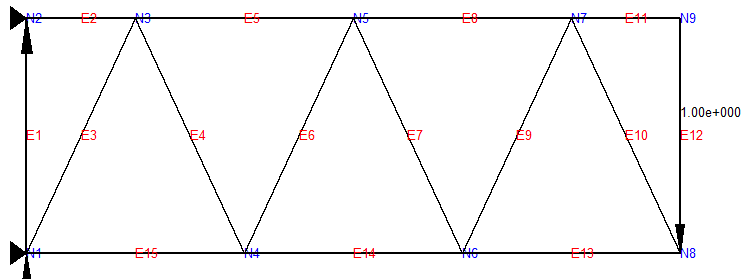
\includegraphics[width=0.8\textwidth]{images/truss3_given}
    \caption{Design Three}
    \label{fig:indeterm_3}
\end{figure*}

\begin{table*}[hp]
	\centering
	\caption{Design Three - Indeterminate Structures Analysis}
	\label{tbl:indeterm_3}
	\vspace{6pt}
	\begin{tabular}{ccc}
		\toprule
		Element & Force (N) & Element Deflection (m) \\
		\midrule
		1 & 1 & 6.578e-8 \\
		2 & 6 & 3.947e-7 \\ 
		3 & 1.4142  & 1.315e-7 \\ 
		4 & 1.4142  & 1.315e-7 \\ 
		5 & 4 & 5.2627e-7 \\ 
		6 & 1.4142  & 1.315e-7 \\ 
		7 & 1.4142 & 1.315e-7 \\ 
		8 & 2 & 2.63e-7 \\ 
		9 & 1.4142 & 1.315e-7 \\ 
		10 & 1.4142  & 1.315e-7 \\ 
		11 & 0 & 0 \\ 
		12 & 0  & 0 \\ 
		13 & 1  & 1.315e-7 \\ 
		14 & 3  & 3.947e-7 \\
		15 & 5 & 6.578e-7 \\
		\bottomrule
	\end{tabular}
\end{table*}

\begin{figure*}[p]
    \centering
    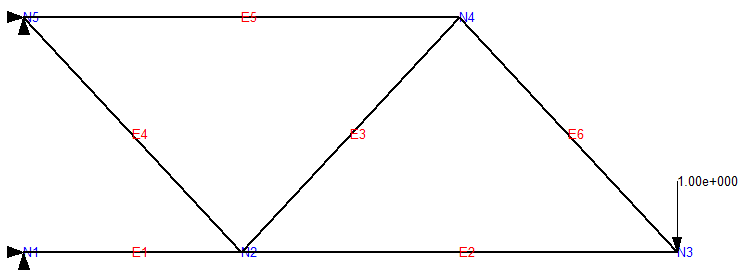
\includegraphics[width=0.8\textwidth]{images/truss5_given}
    \caption{Design Five}
    \label{fig:indeterm_5}
\end{figure*}

\begin{table*}[hp]
	\centering
	\caption{Design Five - Indeterminate Structures Analysis}
	\label{tbl:indeterm_5}
	\vspace{6pt}
	\begin{tabular}{ccc}
		\toprule
		Element & Force (N) & Element Deflection (m) \\
		\midrule
		1 &  -3 &  3.947e-7 \\
		2 &  -1 & 2.63e-7 \\
		3 &  -1.4142 &   2.60e-7 \\
		4 &  1.41421 &  2.63e-7 \\
		5 &  5 & 5.26e-7 \\
		6 &  1.41421 &  2.60e-7 \\ 
		\bottomrule
	\end{tabular}
\end{table*}


\subsection{New Designs} %TODO rename title

Five additional designs were generated to compare against the provided designs.
They may be seen in figures \ref{fig:ours_1}, \ref{fig:ours_2}, \ref{fig:ours_3}, \ref{fig:ours_4} and \ref{fig:ours_5}. %Do 1-5 instead? lol
%how was the first design inspired.
Design seven (figure \ref{fig:ours_2}) was an attempt to improve the most efficient design given (design five) by reducing the material used.
Designs eight and ten (figures \ref{fig:ours_3} and \ref{fig:ours_5}) are similar to the designs provided but have different heights.
The efficiency for each design is presented in table \ref{tbl:stiffness2}
 
 \begin{figure*}[p]
    \centering
    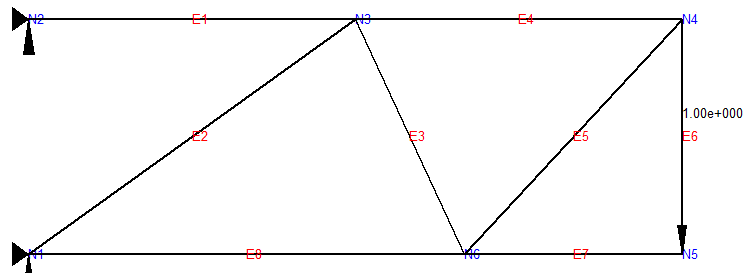
\includegraphics[width=0.6\textwidth]{images/truss1_ours}
    \caption{Design Six}
    \label{fig:ours_1}
\end{figure*}

 \begin{figure*}[p]
    \centering
    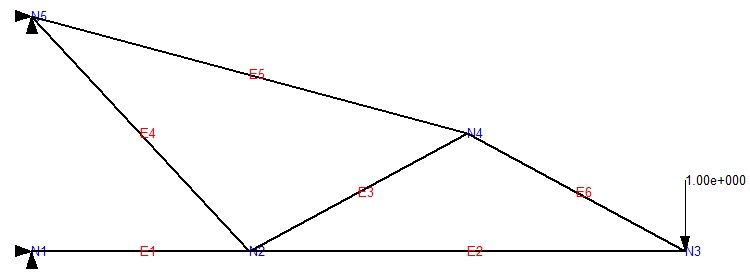
\includegraphics[width=0.6\textwidth]{images/truss2_ours}
    \caption{Design Seven}
    \label{fig:ours_2}
\end{figure*}

 \begin{figure*}[p]
    \centering
    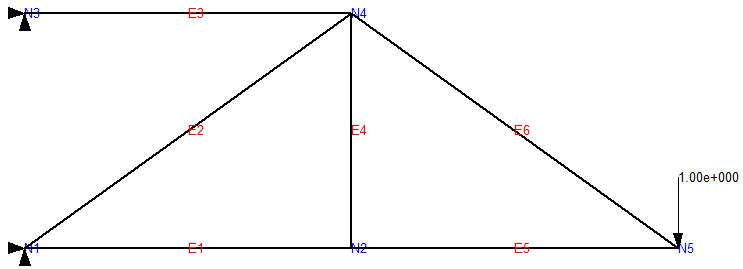
\includegraphics[width=0.6\textwidth]{images/truss3_ours}
    \caption{Design Eight (Height of 10 cm)}
    \label{fig:ours_3}
\end{figure*}

 \begin{figure*}[p]
    \centering
    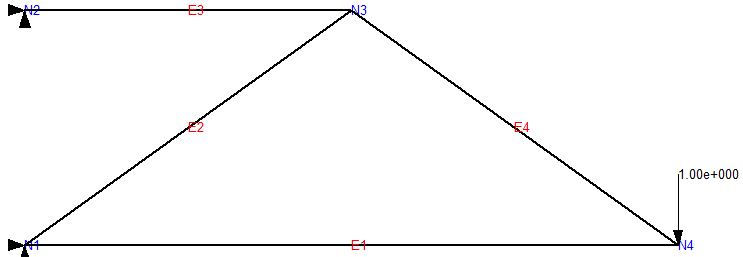
\includegraphics[width=0.6\textwidth]{images/truss4_ours}
    \caption{Design Nine}
    \label{fig:ours_4}
\end{figure*}

 \begin{figure*}[p]
    \centering
    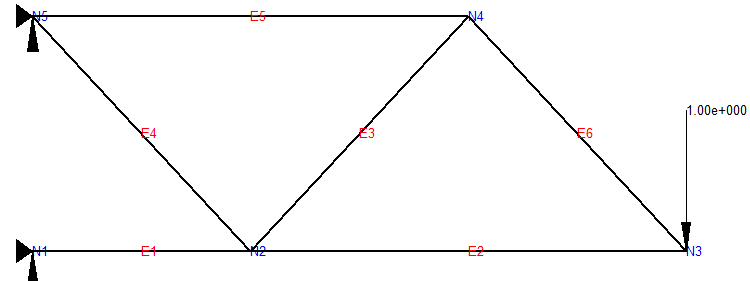
\includegraphics[width=0.6\textwidth]{images/truss5_ours}
    \caption{Design Ten (Height of 5 cm)}
    \label{fig:ours_5}
\end{figure*}


\begin{table*}[hp]
	\centering
	\caption{Stiffness and Efficiency - New Designs (96 GPa)}
	\label{tbl:stiffness2}
	\vspace{6pt}
	\begin{tabular}{lcccccc}
		\toprule
		Design &  \multicolumn{3}{c}{Stiffness} & \multicolumn{3}{c}{Efficiency} \\
		\cmidrule(r){2-4}
		\cmidrule(r){5-7}
		 & Applied Force & Deflection & Stiffness & Material Length & Weight  & Efficiency \\
		\midrule
		6 & 1 N & 0.0133 mm  & 75.2 & 0.991 m & 66.6 g & 1129 \\
		7 & 1 N &  0.0045 mm & 222.7 & 0.871 m & 58.6 g & 3803 \\
		%
		%There has to be something wrong with this:
		8 & 1 N & 0.0017 mm & 602.8 & 0.911 m & 61.2 g & 9848 \\
		%
		9 & 1 N & 0.0042 mm & 237.7 & 0.811 m & 54.5 g &  4364 \\
		10 & 1 N & 0.0122 mm & 82.0 & 0.8354 m & 56.2 g & 1460 \\
		\bottomrule
	\end{tabular}
\end{table*}


\subsection{Discussion}

\subsubsection{Design Features}
%Using your two-dimensional finite element analysis of truss structure behaviours discuss the strengths and weakness of different truss designs and highlight design features that you think will be most effective for your design project. (Your project truss must span 30 cm – from motor shaft to electromagnet center and carry the electromagnet (25 g) and mass (10g) with less than 0.05 mm deflection).

When doing the two-dimensional FEA of the test trusses, we determined that the last design, number 5, was the most efficient truss in terms of deflection and tolerance to buckling. 
We therefore used this truss as a starting point for our truss design. 
The features in design 5 that make for an effective design are maximizing the allowable height, balancing stiffness vs. weight, and ensuring individual truss members have similar safety factors (as is the case for design 5 - Table \ref{tbl:buckling}).   



\subsubsection{3D Structures}
%Discuss the limitations of using a 2D analysis to predict the behaviour of a 3D structure. How will the 3D structure behaviour differ from the 2D? What other concerns do you have for predicting the behaviour of the truss structure? How can you analyze those forces and deflections? (remember, the truss structure will be rotating about one end to move an object as quickly and accurately as possible from point A to point B)

%These sound more like modeling limitations.
%This should be 2d vs 3d (perhaps 3d modeling)

Although the results from 2D behavior resemble closely the 3D behaivor, 2D results are only approximation.
Several assumptions are made to simplify the calculations such as no bending, all joints are pinned and forces act on the same plane. 
The behavior of 3D is not exactly as predicted 2D behavior. However, 2D will give a good indication (approximation) of the magnitudes of the forces and deflection of each member in 3D design.
A 2D analysis will also likely provide a reliable indication of the most efficient 3D structure

\subsubsection{FEM and Indeterminate Structures}
%- Compare the finite element predicted outcomes with your indeterminate structure calculations and discuss the accuracy of each method (keep in mind the assumptions that go into both methods).

The finite element analysis was performed on structure 3, which differed from our values obtained by indeterminate analysis by a factor of 2. 
Accounting for this, our values are within 20\%, which is within an acceptable range.  

\subsubsection{Additional Methods}
%Discuss how you will use these different analysis methods to optimize your final truss design, are there other analysis methods or software that you will use? What are their advantages/disadvantages over the methods used here?

We plan to use 2-D finite element outcomes to tweak our design for optimization as well as indeterminate truss calculations to confirm our FEA results. 
In addition, since our final design will be in 3-D, we will consider using SolidWorks. 
The advantage to this method is that it allows us to visualize different possible 3-D structures and also apply rudimentary finite element analysis to the completed design. 

\subsubsection{Improving Efficiency}
%What else can you do to improve the efficiency of your truss structure?

By the definition of efficiency (stiffness/weight), the two ways to improve efficiency are either to increase the stiffness or reduce the weight.  We discovered that by increasing the height of the truss, to a maximum of 10 cm, we were able to increase the stiffness significantly for a variety of designs. On the other hand, by choosing designs with fewer members, we were able to reduce the overall length of brass rod used and minimize weight.  



\subsection{Conclusion}

It appears the fifth design given proves the best efficiency and has a large factor of safety in all compressive members.
Additional examination of this design will be performed and a 3D model built to validate 2D calculations and assumptions.
More accurate constraints for mounting will also be considered.
Overall, the feature which was found to contribute most to structure efficiency was height.